\chapter{Trabajo Realizado}
\label{chap:Traballo Realizado}

\lettrine{E}{n} este capítulo se presenta el trabajo realizado para adaptar el framework IDIR al registro de imágenes de retina en 2D. Se comienza con una vista general del proceso y una descripción detallada del método IDIR original, seguido de la explicación de las modificaciones realizadas para adaptar el sistema a las características específicas de las imágenes de fondo de ojo. Posteriormente, se describen los conjuntos de datos empleados, el diseño experimental desarrollado y los métodos de evaluación utilizados para validar los resultados.

\section{Vista General}
\label{sec:VistaXeral}

El trabajo realizado se centró en la adaptación del framework IDIR, originalmente diseñado para 4D-CT torácicas, al problema específico del registro de imágenes de fondo de ojo en 2D. Esta tarea requirió modificar la arquitectura de la red neuronal para operar en dos dimensiones, reformular los términos de regularización y adaptar los procesos de entrenamiento y evaluación para el nuevo dominio.
Para optimizar el modelo, se diseñó un proceso de experimentación sistemático y se desarrollaron metodologías de entrenamiento específicas. Entre ellas destacan la creación de estrategias de muestreo que priorizan regiones de interés anatómico y técnicas como el ajuste dinámico de hiperparámetros para refinar la convergencia del modelo.

Finalmente, para validar los resultados, se construyó un marco de evaluación que fue aplicado sobre los datasets FIRE (que contiene pares de imágenes reales con diferentes grados de superposición y variaciones anatómicas) y RFMiD (transformaciones lineales generadas), lo que permite juzgar distintas características de la red. La evaluación combinó métricas cuantitativas objetivas y el análisis cualitativo visual para garantizar la calidad y el realismo de las deformaciones obtenidas.

\section{IDIR}
\label{sec:IDIR}

IDIR (Implicit Deformable Image Registration) es un método de alineamiento de imágenes basado en redes neuronales.
Su principal diferencia frente a una red convolucional tradicional es que,

Lo que se propone es optimizar directamente el DFV haciendo uso de una representación implícita, de forma que la deformación está representada en los propios pesos de un MLP \cite{wolterink2021implicit}.

Otros trabajos como NIR \cite{sun2024medicalimageregistrationneural} o NODEO \cite{nodeo} proponen métodos de registro similares que también hacen uso de representaciones implícitas de las deformaciones, aplicados a resonancias magnéticas del cerebro.

\subsection{Arquitectura}
\label{subsubsec:Arquitectura}

Se hace uso de un MLP de 3 capas, y determinaron experimentalmente que obtenían mejor resultado con 256 unidades por capa que 128.
Por cada época de entrenamiento (2500 en total), 10000 puntos son muestreados aleatoriamente del espacio de coordenadas dentro de la máscara.
El término de pérdida es la 'normalized cross-correlation' entre los valores de los píxeles muestreados en la imagen fija y los correspondientes de la imagen móvil.
Utilizan Adam de optimizador, con un learning rate de 0.0001.

\subsubsection{Función de activación}
\label{subsubsec:Función de activación}

Una elección estándar para la función de activación es \textbf{ReLU}:

\[
f(x) = \max(0, x) = \begin{cases} 
x & \text{si } x > 0 \\ 
0 & \text{si } x \leq 0 
\end{cases}
\]

No obstante, para redes de representación implícita como con la que estamos trabajando, esta tiene una serie de desventajas.

Las ReLUs tienen un sesgo hacia señales de baja frecuencia \cite{rahaman2019spectralbiasneuralnetworks},
lo que significa que el modelo puede tener dificultades para representar pequeñas deformaciones locales en el registro de imágenes.

\cite{ziyin2020neuralnetworksfaillearn} demostraron que la gran parte de las funciones de activación utilizadas en redes neuronales (ReLU, tanh, sigmoide y todas sus variantes)
son incapaces de extrapolar funciones periódicas sencillas debido a su tendencia a converger hacia comportamientos lineales cuando se extrapolan fuera del rango de entrenamiento.

Existen varias formas de superar este sesgo, como preprocesar las coordenadas de entrada con funciones de activación periódicas \cite{mildenhall2020nerfrepresentingscenesneural}
o sustituir la función de activación ReLU por una función de activación periódica \cite{sitzmann2020implicitneuralrepresentationsperiodic}.

En este trabajo escogemos la segunda opción, utilizando una función de activación periódica de tipo \textbf{SIREN}:

\[
f(x) = \sin(ax + b), \quad \text{con} \quad a, b \in \mathbb{R}
\]

Una ventaja añadida de las funciones de activación periódicas en las redes SIREN es que pueden ser diferenciadas varias veces,
lo que expande sustancialmente el conjunto de términos de regularización que se pueden emplear en la red, como veremos en la siguiente sección.

larger frequencies appear in the networks for weights with larger magnitudes.

Otros trabajos como \cite{mildenhall2020nerfrepresentingscenesneural} no utiliza una función de activación periódica, pero para la representación adecuada de zonas de alta frecuencia
utilizaron codificación posicional, que ya las incorpora de forma implícita en la red con buenos resultados.

Otra de las ventajas que tiene SIREN es que es una función suave o infinitamente diferenciable, es decir, que admite derivadas de cualquier orden.
Otros ejemplos de funciones de activación infinitamente diferenciables son:

Sigmoide:
\[
f(x) = \frac{1}{1 + e^{-x}}
\]
Tangente Hiperbólica:
\[
f(x) = \tanh(x) = \frac{e^x - e^{-x}}{e^x + e^{-x}}
\]

Softplus:
\[
f(x) = \ln(1 + e^x)
\]

\paragraph{Inicialización de pesos}

En \cite{sitzmann2020implicitneuralrepresentationsperiodic} propusieron una inicialización específica para las redes SIREN,
la cual consiste en inicializar la primera capa de modo que la función seno recorra múltiples períodos sobre el intervalo [−1,1][−1,1].
Esto se consigue multiplicando los pesos de la primera capa por un factor de escala ω0, sobre el cual recomiendan ω0=30.
La fórmula para la inicialización de los pesos de la primera capa es la siguiente:

\begin{figure}[tbp]
    \centering
    \[
    w_i \sim U\left[ -\frac{1}{n}, \frac{1}{n} \right]
    \]

\caption{Inicialización primera capa}
\end{figure}

donde n es el número de neuronas de entrada (el tamaño de la capa anterior).

Las siguientes capas se inicializan de la siguiente forma:
\begin{figure}[tbp]
    \centering
    \[
    w_i \sim U\left[ -\frac{\sqrt{\frac{6}{n}}}{w}, \frac{\sqrt{\frac{6}{n}}}{w} \right]
    \]
    \caption{Inicialización siguientes capas}
\end{figure}

De esta forma se asegura que la entrada a cada activación sinusoidal está distribuida normalmente con una desviación estándar de 1,
lo que debería mejorar la estabilidad y convergencia durante el entrenamiento de la red.
Una consecuencia de esto es que, ya que los propios pesos de la red representan la deformación, inicialmente la red comienza con una deformación muy similar en todos los casos, que el entrenamiento deberá corregir.

En \cite{sireninit} implementan una versión simplificada de SIREN para facilitar el estudio de estas,
y proponen mejoras en el proceso de inicialización. Una de ellas es utilizar la distribución Kaiming (He) en lugar de la uniforme.
También proponen un método para escoger un valor de w apropiado según el problema a resolver.

\subsubsection{Términos de Pérdida}\label{subsubsec:Termos de Perda}

El término de pérdida es la función que se optimiza durante el entrenamiento, y es lo que guía la red hacia una solución óptima.
Esta cuantifica la discrepancia entre la salida de la red y el resultado deseado.

Para la tarea de registro de imágenes, se utilizan dos categorías principales de métricas para evaluar la alineación entre imágenes:
las métricas basadas en el error y las métricas basadas en la similitud. Las métricas basadas en el error (MSE, L1...) miden las diferencias píxel a píxel entre las imágenes,
siendo más sensibles a diferencias locales y proporcionando una medida absoluta.
Las métricas basadas en la similitud (NCC, SSIM...) tienen en cuenta patrones estructurales y relaciones estadísticas entre las imágenes, siendo más robustas frente a variaciones en la iluminación y pequeños desplazamientos.
\cite{simmetric}

Los principales términos de pérdida valorados para este trabajo son:

\begin{itemize}
    % Error-based metrics
    \item \textbf{MSE (Mean Squared Error)}:
    Error cuadrático promedio entre la imagen fija y la móvil. Es sensible a valores atípicos y ruido.
    \[
    \text{MSE} = \mathbb{E}[(Y - \hat{Y})^2] = \frac{1}{N} \sum_{i=1}^{N} (y_i - \hat{y}_i)^2
    \]
    donde \( y_i \) es el valor del píxel de la imagen fija, \( \hat{y}_i \) es el valor del píxel de la imagen móvil, y \( N \) es el número total de píxeles. \cite{Palubinskas02012017}

    Regularizador Hiperelástico en 2D   \item \textbf{L1 (Mean Absolute Error)}:
    Mide el error absoluto promedio. Menos sensible a valores atípicos que MSE.
    \[
    \text{L1} = \mathbb{E}[|Y - \hat{Y}|] = \frac{1}{N} \sum_{i=1}^{N} |y_i - \hat{y}_i|
    \]

    % Robust error metrics
    \item \textbf{Huber Loss}:
    Combina MSE y L1, siendo cuadrática para errores pequeños y lineal para errores grandes.
    \[
    \text{Huber}(y, \hat{y}) = \begin{cases}
    \frac{1}{2}(y - \hat{y})^2 & \text{si } |y - \hat{y}| \leq \delta \\
    \delta(|y - \hat{y}| - \frac{1}{2}\delta) & \text{en otro caso}
    \end{cases}
    \]
    donde \( \delta \) es un hiperparámetro que define el punto de transición entre los comportamientos cuadrático y lineal.

    \item \textbf{Smooth L1 Loss}:
    Similar a Huber Loss, pero con una transición suave entre las regiones cuadrática y lineal.
    \[
    \text{SmoothL1}(y, \hat{y}) = \begin{cases}
    \frac{1}{2}(y - \hat{y})^2 & \text{si } |y - \hat{y}| \leq 1 \\
    |y - \hat{y}| - \frac{1}{2} & \text{en otro caso}
    \end{cases}
    \]

    % Similarity-based metrics
    \item \textbf{NCC (Normalized Cross-Correlation)}:
    Evalúa la similitud entre las dos imágenes normalizando sus intensidades. Es invariante a cambios en la iluminación.
    \[
    \text{NCC} = \frac{\sum_{i=1}^{N} (y_i - \mu_y)(\hat{y}_i - \mu_{\hat{y}})}{\sqrt{\sum_{i=1}^{N} (y_i - \mu_y)^2 \sum_{i=1}^{N} (\hat{y}_i - \mu_{\hat{y}})^2}}
    \]
    donde \( \mu_y \) y \( \mu_{\hat{y}} \) son las medias de las imágenes fija y móvil, respectivamente.

    \item \textbf{SSIM (Structural Similarity Index)}:
    Evalúa la similitud estructural entre las dos imágenes, considerando luminancia, contraste y estructura.
    \[
    \text{SSIM}(y, \hat{y}) = \frac{(2\mu_y\mu_{\hat{y}} + C_1)(2\sigma_{y\hat{y}} + C_2)}{(\mu_y^2 + \mu_{\hat{y}}^2 + C_1)(\sigma_y^2 + \sigma_{\hat{y}}^2 + C_2)}
    \]
    donde \( \mu_y \), \( \mu_{\hat{y}} \) son las medias, \( \sigma_y \), \( \sigma_{\hat{y}} \) son las desviaciones estándar, \( \sigma_{y\hat{y}} \) es la covarianza, y \( C_1 \), \( C_2 \) son constantes para evitar divisiones entre cero. \cite{Palubinskas02012017}
\end{itemize}

Debido a la naturaleza de las imágenes de retina, donde pueden existir diferencias de iluminación y contraste entre las imágenes fija y móvil,
parece más apropiado emplear métricas basadas en la similitud como NCC o SSIM.

NCC se utilizó la implementación de https://github.com/BDdeVos/TorchIR/blob/main/torchir/metrics.py.

\subsubsection{Términos de regularización}\label{subsubsec:Termos de regularización}

Debido a que el registro de imágenes deformables es un problema mal formulado (ill-posed problem),
es común utilizar algún tipo de regularización sobre el DVF para evitar deformaciones poco realistas.
Los métodos de registro basados en redes neuronales convolucionales (CNN) representan los DVFs
como muestras en una cuadrícula de vóxeles, y por lo tanto, solo se pueden aproximar gradientes espaciales
mediante esquemas de diferencias finitas (aproximar derivadas mediante cálculo numérico de diferencias entre valores adyacentes en la cuadrícula).
Este es un proceso computacionalmente muy costoso e ineficiente, además implica errores de discretización y pérdidas de precisión.

Haciendo uso de representaciones implícitas, todas las operaciones son diferenciables, y los gradientes pueden
ser computados fácilmente de forma analítica en lugar de tener que aproximarlos, haciendo uso de la librería de autodiferenciación de PyTorch.

Utilizando ReLU como función de activación, la red es diferenciable una vez, mientras que utilizando
una función de activación periódica (como SIREN), la red es diferenciable todas las veces que se precise.
De esta forma, podemos calcular cualquier número de términos de regularización e incluirlos en la optimización de la red.

Algunos ejemplos de términos de regularización que se pueden emplear son:
\begin{itemize}
    \item Jacobian regularizer: 
    El determinante Jacobiano de la transformación (det ∇Φ) en una localización x es un indicador de estiramiento o compresión local.
    Un determinante Jacobiano negativo o muy cercano a 0 indica que están ocurriendo pliegues y la transformación no será invertible.
    La matriz jacobiana es la matriz que contiene todas las derivadas parciales de la función de transformación (calculado mediante gradientes).
    El término de regularización del Jacobiano penaliza los valores del determinante Jacobiano que se desvían de 1,
    intentando preservar áreas locales y evitar estiramientos o pliegues extremos.

    \begin{figure}[tbp]
        \centering
        \[
        S^{jac}[\Phi] = \int_{\Omega} \left| 1 - \det \left( \nabla \Phi \right) \right| \, dx
        \]
        \caption{Regulizador Jacobiano}
    \end{figure}

    Ω representa el dominio o región del espacio sobre el cual está definida la transformación Φ.
    
    \item Hyperelastic regularizer
    También se pueden añadir restricciones al DVF con este término propuesto por \cite{HyperelasticRegularization}.
    Consiste en tres términos, un término de longitud, un término de área y un término de volumen con el objetivo de controlar variaciones en estos aspectos.
    El término de longitud penaliza la variación de la longitud de los vectores del DVF, siendo u la medida desplazamiento de un punto en el espacio.
    La matriz de cofactores de la matriz del Jacobiano de la transformación controla el área,
    La función de máximo asegura que solo las expansiones que sobrepasen cierto límite sean penalizadas
    El determinante de la matriz del Jacobiano controla el volumen,
    y ambas penalizan el crecimiento y la contracción por igual.
    αl, αa y αν son hiperparámetros que controlan la importancia de cada término.

    \begin{figure}[tbp]
        \centering
        \[
        S^{hyper}[\Phi] = \int_{\Omega} \left[ \frac{1}{2} \alpha_1 |\nabla u|^2 + \alpha_a \varphi_c (\text{cof} \nabla \Phi) + \alpha_\nu \psi(\det \nabla \Phi) \right] dx,
        \]
        \[
        \text{Funciones convexas:} \quad \varphi_c(C) = \sum_{i=1}^3 \max \left\{ \sum_{j=1}^3 C_{ji}^2 - 1, 0 \right\}^2 \quad \text{and} \quad \psi(v) = \frac{(v-1)^4}{v^2}.
        \]
        \caption{Regulizador Hiperelástico.}
    \end{figure}


    \item Bending energy penalty
    Se puede imponer la suavidad de la deformación empleando esta penalización propuesta en \cite{bendingenergy}, que
    requiere que las segundas derivadas del DVF sean pequeñas en todo el dominio, lo que evita deformaciones bruscas y discontinuas.
    Este término no puede ser utilizado en una red que utilice ReLU como función de activación, ya que la segunda derivada de una ReLU es siempre igual a 0.

    \begin{figure}[tbp]
        \centering
        \[
        S^{bending}[\Phi] = \frac{1}{8} \int_{-1}^{1} \int_{-1}^{1} \int_{-1}^{1} \left[ \left( \frac{\partial^2 \Phi}{\partial x^2} \right)^2 + \left( \frac{\partial^2 \Phi}{\partial y^2} \right)^2 + \left( \frac{\partial^2 \Phi}{\partial z^2} \right)^2 \right.
        \]
        \[
        \left. + 2 \left( \frac{\partial^2 \Phi}{\partial x \partial y} \right)^2 + 2 \left( \frac{\partial^2 \Phi}{\partial x \partial z} \right)^2 + 2 \left( \frac{\partial^2 \Phi}{\partial y \partial z} \right)^2 \right] dx\,dy\,dz
        \]
        \caption{Regulizador Bending Energy}
    \end{figure}
    
\end{itemize}

Para la implementación en este trabajo se modificaron todos estos términos para que funcionaran con transformaciones de dos dimensiones en lugar de tres,
sustituyendo el gradiente de 3 dimensiones en el Jacobiano por uno de dos, eliminando las derivadas parciales en z en bending energy y el término de volumen en el término hiperelástico.

\begin{itemize}
    \item Jacobian regularizer:\\
    \[
    S^{jac}[\Phi] = \int_{\Omega} \left| 1 - \det \left( \nabla \Phi \right) \right| \, dx \, dy
    \]
    \item Hyperelastic regularizer:\\
    \[
    S^{hyper}[\Phi] = \int_{\Omega} \left[ \frac{1}{2} \alpha_1 |\nabla u|^2 + \alpha_a \varphi_c (\text{cof} \nabla \Phi) \right] dx \, dy,
    \]
    \[
    \varphi_c(C) = \sum_{i=1}^2 \max \left\{ \sum_{j=1}^2 C_{ji}^2 - 1, 0 \right\}^2
    \]
    \item Bending energy penalty:\\
    \[
    S^{bending}[\Phi] = \frac{1}{8} \int_{-1}^{1} \int_{-1}^{1} \left[ \left( \frac{\partial^2 \Phi}{\partial x^2} \right)^2 + \left( \frac{\partial^2 \Phi}{\partial y^2} \right)^2 + 2 \left( \frac{\partial^2 \Phi}{\partial x \partial y} \right)^2 \right] dx \, dy
    \]
\end{itemize}

La regularización también tiene un impacto significativo en el tiempo de computación, ya que requiere múltiples pasadas de retropropagación por época para calcular los distintos términos de penalización.
Sin regularización solo se hace 1 pasada para calcular el gradiente del término de similitud de la imagen.
Con la regularización del Jacobiano, además del término de similitud, se calculan dos derivadas (una por dimensión) para obtener el Jacobiano, resultando en 3 pasadas por época.
Añadiendo la regularización hiperelástica (sin término de volumen), es necesario calcular una derivada adicional para el cofactor de la matriz Jacobiana, haciendo un total de 4 pasadas por época.
Finalmente, con la penalización de energía de flexión, se necesitan derivadas segundas, lo que implica 7 pasadas por época en total.
En el trabajo original de IDIR, llegaban a usar 13 pasadas debido a que trabajan en 3D.

Si los términos de regularización tienen demasiada influencia sobre el término de pérdida, la red hará transformaciones muy pequeñas para evitar ser penalizada, lo que resultará en una transformación insuficiente.
Por otro lado, si los términos son demasiado pequeños, la red hará transformaciones muy grandes, lo que resulta en una transformación irrealista y sobreajustada. Esto es especialmente evidente en el caso de la función de activación SIREN, que tiende a sobreajustarse fácilmente debido a su sesgo hacia señales de alta frecuencia.
La cantidad óptima de regularización depende de la pareja concreta de imágenes a alinear, por lo que intentaremos determinar cuál es la mejor para una muestra de imágenes.

Además, pese a que los diferentes términos de regularización valoran diferentes aspectos, cabe tener en cuenta que también hay superposición en algunas de las propiedades que valoran.
Por ejemplo, el regularizador hiperelástico puede considerarse un término más general que incluye indirectamente penalizaciones del Jacobiano (ambos penalizan los "pliegues") y de suavidad de las transformaciones (como hace el bending pero en menor grado).

\subsubsection{Learning rate y tamaño de lote}
\label{subsubsec:Learning rate e tamaño de lote}

El learning rate es un parámetro del optimizador (Adam en este caso) que regula el tamaño de los ajustes efectuados a los parámetros del modelo durante cada iteración de actualización.
Determina la magnitud del cambio aplicado para minimizar la función de pérdida, afectando tanto a la velocidad de convergencia como a la estabilidad del proceso de aprendizaje.
Un learning rate demasiado alto puede provocar que la red diverja, mientras que un learning rate demasiado bajo puede resultar en convergencia lenta o quedar atrapado en mínimos locales.

Debido a la naturaleza de la red, el tamaño de lote utilizado tiene una relación directa con el learning rate, por lo que intentaremos determinar la relación óptima entre ambos.

Una de las heurísticas más comunes para relacionar el learning rate y el tamaño de lote es la regla de escalado lineal \cite{goyal2018accuratelargeminibatchsgd}.
La regla indica que el learning rate óptimo debe escalarse linealmente con la cantidad de muestras por lote.

Una forma de explicar esto es, ya que con tamaños de lote más grandes tenemos una mejor aproximación del gradiente real, es posible utilizar un learning rate mayor sin que la red diverja. \cite{kexuefm}

El tamaño de lote en esta red representa el número de coordenadas muestreadas aleatoriamente del espacio de coordenadas dentro de la máscara.

\subsection{Método}\label{subsubsec:Método}

Siendo el objetivo encontrar una transformación espacial óptima entre la imagen móvil y la imagen fija,
es necesario obtener la función de deformación Φ(x) = u(x) + x que mapea cada coordenada x en la imagen móvil a una coordenada en la imagen fija,
de forma que la coordenada x en la imagen fija corresponda anatómicamente a la coordenada Φ(x) en la imagen móvil.
Este problema puede ser formulado como un problema de optimización donde $L_{data}$ es una métrica de similitud entre las imágenes fija ($F$) y móvil ($M$), $L_{reg}$ es un término de regularización en la transformación Φ, y α es un término de ponderación.
\begin{equation}
    \hat{\Phi} = \operatorname*{Arg\,min}_{\Phi} L_{data}(M \circ \Phi, F) + \alpha L_{reg}(\Phi)
\end{equation}

La principal innovación que introduce IDIR\cite{wolterink2021implicit} es que la transformación Φ está implícitamente representada en la red neuronal.

Comparado con una CNN tradicional, esta red no recibe valores de intensidad de píxel como entrada,
sino que recibe coordenadas espaciales (continuas) y devuelve una nueva coordenada.
Ya que los pesos de la red definen la transformación, estos pueden ser optimizados directamente
haciendo uso de una métrica de similitud como función de pérdida.

Parametrizar la función de deformación como una \glossary{INR} dentro de un \glossary{MLP} tiene varias ventajas para el registro de imágenes.
En primer lugar, la representación de la transformación es continua y por lo tanto independiente de la resolución de la imagen,
gracias a ello el mismo modelo puede ser empleado para imágenes de cualquier tamaño, al contrario de una CNN tradicional
que tiene que ser adaptada para cada resolución.

Segundo, hacerlo de esta forma permite aprovechar las capacidades de librerías como PyTorch para calcular los gradientes de la transformación respecto a las coordenadas.
Esto permite obtener gradientes más precisos que las aproximaciones por diferencias finitas
y permite aprovechar una gran cantidad de literatura sobre regularización eficientes en imágenes médicas.

Tercero, se puede modificar la función de activación empleada en la red para ajustarla a las necesidades particulares de la tarea de registro de imágenes.

El \gls{NTK} describe cómo un modelo de red neuronal responde a cambios en sus parámetros durante el entrenamiento,
y dependiendo de la función de activación empleada, el NTK varía y la red puede ser más o menos sensible a ciertas deformaciones.

Finalmente, se entrenará una nueva red por cada pareja de imágenes, siendo esta una red bastante pequeña en comparación y prescindiendo de la necesidad de grandes conjuntos de datos para su entrenamiento.

\subsection{Replicación de resultados}
\label{subsec:Replicación de resultados}

Se replicaron los resultados obtenidos por Wolterink et al. \cite{wolterink2021implicit} que se muestran en la tabla \ref{tab:comparison}.

\begin{table}[ht]
    \centering
    \caption{Replicación de los resultados de IDIR}
    \begin{tabular}{c|c}
        Scan & {IDIR / Replicación} \\
        1  & 0.76 (0.94) / 0.79 (0.92) \\
        2  & 0.76 (0.94) / 0.71 (0.89) \\
        3  & 0.94 (1.02) / 0.95 (1.01) \\
        4  & 1.32 (1.27) / 1.32 (1.22) \\
        5  & 1.23 (1.47) / 1.23 (1.46) \\
        6  & 1.09 (1.03) / 1.15 (1.04) \\
        7  & 1.12 (1.00) / 1.11 (0.99) \\
        8  & 1.21 (1.29) / 1.20 (1.28) \\
        9  & 1.22 (0.95) / 1.16 (0.99) \\
        10 & 1.01 (1.05) / 1.09 (1.05) \\
        Promedio & 1.07 / 1.07 (1.08) \\
    \end{tabular}
    \label{tab:comparison}
\end{table}

\section{Adaptación a 2D}
\label{sec:Adaptación a 2D}

Para adaptar el modelo IDIR a 2D, es necesario modificar la arquitectura de la red para que funcione con imágenes bidimensionales.
La arquitectura original de IDIR tiene una entrada de 3 dimensiones (x, y, z) y una salida de 3 dimensiones (dx, dy, dz),
mientras que nuestra red tiene una entrada de 2 dimensiones (x, y) y una salida de 2 dimensiones (dx, dy).

Se modificaron las capas de entrada y salida de la red para que acepten coordenadas bidimensionales (originalmente [3, 256, 256, 256, 3], ahora [2, 256, 256, 256, 2]).

Fue necesario modificar las funciones de interpolación, que antes interpolaban valores tridimensionales y ahora interpolan valores bidimensionales.

También se adaptaron los términos de regularización para que funcionen con coordenadas bidimensionales, como se detalla en la sección \ref{subsubsec:Termos de regularización}.

Finalmente, el proceso de evaluación tuvo que implementarse desde 0 para adaptarse al nuevo formato de imágenes y datos de referencia.

\subsection{Proceso de Registro}
\label{subsec:Proceso de Registro}

El registro de cada par de imágenes (fija y móvil) se trata como un problema de optimización independiente. Para cada par, se entrena una nueva red neuronal desde cero cuyo único objetivo es aprender la deformación específica que alinea esas dos imágenes.

Primeramente, se crea una instancia del MLP con la arquitectura 2D y se definen los hiperparámetros como la función de activación, la métrica de pérdida y términos de regularización que se aplicarán. La inicialización de los pesos de la red es un paso de especial relevancia.

Una vez inicializada la red, se genera un tensor de coordenadas que contiene la localización (x, y) de todos los píxeles que se encuentran dentro de la máscara de la imagen fija. Este tensor representa el espacio de coordenadas completo sobre el que la red aprenderá la deformación.

A continuación, comienza el bucle de entrenamiento, que se repite durante un número predefinido de épocas. En cada iteración dentro de una época, se realiza el siguiente proceso:
\begin{itemize}
    \item \textbf{Muestreo de Coordenadas:} En lugar de procesar la imagen entera en cada paso, se selecciona un subconjunto de puntos del tensor de coordenadas igual al tamaño de lote. La estrategia de muestreo es un componente crítico que fue objeto de experimentación en este trabajo.

    \item \textbf{Predicción y Aplicación de la Transformación:} Las coordenadas (x, y) muestreadas se introducen en la red. El MLP actúa como una función de deformación implícita, devolviendo para cada coordenada de entrada un vector de desplazamiento (dx, dy).

    \item \textbf{Cálculo de la Pérdida (Loss):} Para cuantificar lo bien que la deformación alinea las imágenes, se comparan los valores de intensidad en los puntos seleccionados. Para cada coordenada original $(x,y)$ en la imagen fija, se obtiene el valor de intensidad correspondiente en la imagen móvil en la coordenada transformada $(x + dx, y + dy)$. Como esta última suele ser una posición no entera, se utiliza interpolación para estimar su valor de intensidad. La métrica de pérdida (NCC, SSIM, etc.) calcula la discrepancia entre el conjunto de intensidades de la imagen fija y el de las intensidades obtenidas de la imagen móvil transformada.

    \item \textbf{Retropropagación y Actualización:} Al valor de la pérdida de similitud se le suman los términos de penalización calculados a partir de los regularizadores. El valor de pérdida total resultante se utiliza para calcular los gradientes respecto a los pesos de la red mediante retropropagación. Finalmente, el optimizador (Adam) utiliza estos gradientes para actualizar los pesos del MLP, ajustándolos ligeramente en la dirección que minimiza la pérdida.
\end{itemize}

Este ciclo se repite hasta completar todas las épocas. Al final del entrenamiento, los pesos optimizados de la red encapsulan la función de deformación continua y específica para ese par de imágenes.

Es crucial subrayar que la tarea de registro de retinografías difiere sustancialmente de la de pulmones. Por este motivo, no es posible asumir que los hiperparámetros óptimos del trabajo original sean válidos para este nuevo dominio, lo que justifica la extensa experimentación realizada.

\section{Conjuntos de datos}
\label{sec:Conjuntos de datos}

\subsection{FIRE}
\label{subsec:FIRE}

Está compuesto por 134 pares de imágenes de retinas, con un tamaño de 2912 × 2912 píxeles y un \gls{FOV} de 45◦× 45◦.
Están clasificadas en 3 categorías según el grado de superposición y la presencia de diferencias anatómicas: \textit{S}, \textit{P} y \textit{A}. \cite{FIRE}

\begin{figure}[tbp]
    \centering
    \setlength{\tabcolsep}{8pt} % Adjust column spacing
    \begin{tabular}{|c|c|c|c|}
        \hline
        \textbf{Categoría} & \textbf{Nº de pares de imágenes} & \textbf{Superposición (\%)} & \textbf{Diferencias Visuales} \\
        \hline
        \textbf{\textit{\textsf{S}}} & 71 & > 75 & No \\
        \hline
        \textbf{\textit{\textsf{P}}} & 49 & < 75 & No \\
        \hline
        \textbf{\textit{\textsf{A}}} & 14 & > 75 & Sí \\
        \hline
    \end{tabular}
    \caption{Clasificación de los pares de imágenes en categorías.}
    \label{tab:categorias}
\end{figure}
\FloatBarrier

Incluye 10 puntos de referencia para cada imagen, que se utilizan para la evaluación del registro, así como una máscara por cada imagen que indica la localización de los píxeles con información de color.

\begin{figure}[tbp]
    \centering
    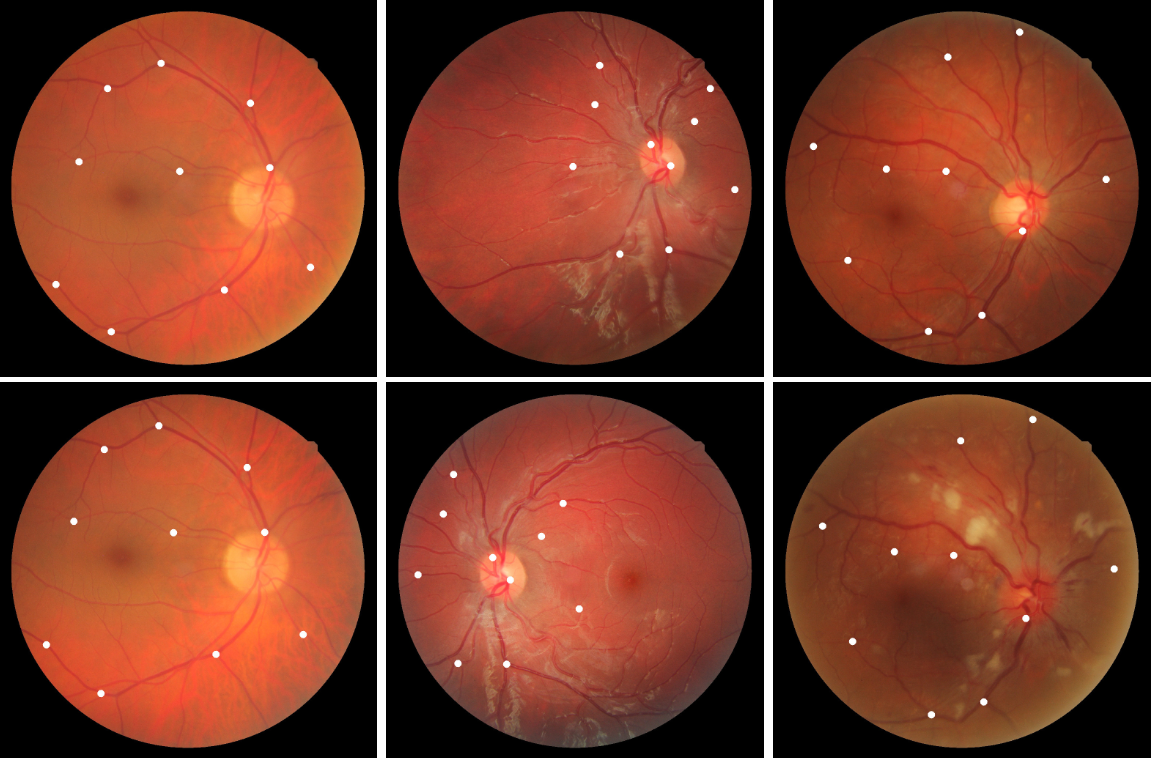
\includegraphics[width=0.8\textwidth]{imaxes/fire-ej.png}
    \caption{Ejemplo de imágenes del conjunto de datos FIRE \cite{FIRE} con los puntos de control indicados. De izquierda a derecha, categorías \textit{\textsf{S}}, \textit{\textsf{P}}, \textit{\textsf{A}} .}
    \label{fig:fire_ej}
\end{figure}

\subsection{RFMID}\label{subsec:RFMID}

El conjunto de datos RFMiD \cite{RFMiD} proporciona 3200 imágenes de fondo de ojo en color con resolución 1712x1712, etiquetadas según si tienen alguna anomalía o no.
También proporciona etiquetas para 45 diferentes anomalías anotadas por expertos.

Para utilizarlo en este trabajo, seleccionamos una submuestra y generamos transformaciones aleatorias. Guardamos las imágenes originales y las transformadas así como las matrices de transformación asociadas para la posterior evaluación.
También se divide entre transformaciones de color y de geometría.

En la figura \ref{fig:rfmid_ej} se muestra un ejemplo de una pareja de imágenes del conjunto de datos RFMiD.

\begin{figure}[tbp]
    \centering
    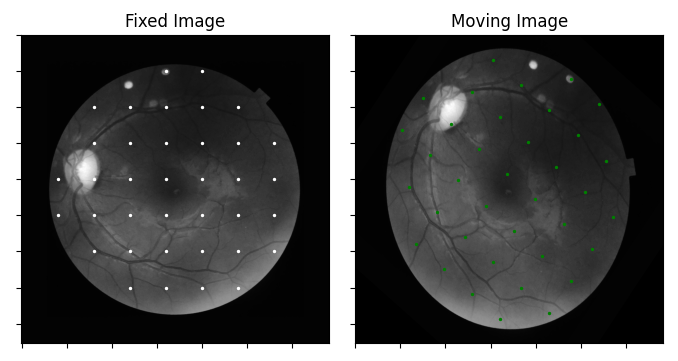
\includegraphics[width=0.8\textwidth]{imaxes/rfmid_ej.png}
    \caption{Ejemplo de imágenes del conjunto de datos RFMiD. La imagen de la izquierda es la fija y la de la derecha es la móvil.}
    \label{fig:rfmid_ej} 
\end{figure} 

\subsection{Diferencias entre los datasets}
\label{subsec:Diferencias entre os datasets}

Una ventaja de utilizar dos conjuntos de datos diferentes es que cada uno de ellos tiene características únicas que permiten evaluar el modelo en diferentes contextos.
La principal diferencia es que RMiFD es un conjunto de datos sintético, en el cual no introducimos diferencias de color y siempre tienen una superposición del 100\%, por lo que lo único que se evalúa es la capacidad del modelo para realizar los registros geométricos.
Por el contrario, FIRE es un conjunto de datos real, en el cual existen cambios en la iluminación, contraste, superposición y demás diferencias visuales, por lo que se evalúa la capacidad del modelo para realizar registros en condiciones mucho más adversas.

\section{Diseño de Experimentos}
\label{sec:Diseño de Experimentos}

El diseño de experimentos es un proceso sistemático que busca determinar la influencia de diferentes factores sobre un resultado específico. En este caso, el objetivo es evaluar cómo diferentes parámetros afectan a la calidad del registro de imágenes.

El coste computacional es un factor muy importante a tener en cuenta, ya que cada combinación de parámetros requiere un entrenamiento completo de la red por cada pareja de imágenes, lo que implica un alto coste energético y de tiempo.
Por ejemplo, para probar una combinación de parámetros sobre FIRE habrá que entrenar una red por cada pareja de imágenes de las 134 del conjunto de datos.
A un tiempo de entrenamiento de 3 minutos por pareja, el entrenamiento completo llevaría más de 6 horas por cada combinación de parámetros, con una huella de memoria de alrededor de 5 GB de VRAM.
El coste temporal y de memoria dependen de varios factores, siendo los más relevantes la regularización empleada, la resolución de la imagen, el tamaño del lote y la función de activación.
En concreto, SIREN tiene un coste computacional mucho mayor que ReLU, requiriendo alrededor del doble de tiempo y memoria para entrenar la red.

Debido al gran número de factores a tener en cuenta, se adoptó un enfoque de experimentación en fases.

Inicialmente se realizaron experimentos iniciales para identificar los rangos de parámetros más prometedores utilizando una submuestra representativa de 14 parejas de imágenes de cada categoría del dataset FIRE, con el objetivo: Reducir el espacio de parámetros para las fases posteriores.
En esta fase se evaluó la métrica de pérdida, la resolución de la imagen, la regularización empleada y el tamaño del lote.

Basándose en los resultados de la primera fase, se realizó una experimentación más exhaustiva para intentar mejorar el rendimiento del registro, centrándose en la estrategia de muestreo, la inicialización de los pesos de la red y un ajuste dinámico del tamaño de lote.

\subsection{Metodologías Desarrolladas}
\label{subsec:Metodoloxías Desenvoltas}

Para este trabajo tuvieron que desarrollarse varias metodologías específicas con el objetivo de mejorar el rendimiento del registro de imágenes de retina. Estas metodologías incluyen:

\subsubsection{Estrategias de Muestreo}
\label{subsubsec:estratexias_mostraxe}

\paragraph{Muestreo Inteligente}
En la estrategia de muestreo inteligente, se calcula una máscara de probabilidad para cada imagen, que se utiliza para seleccionar los puntos que se pasan a la red. Para calcular esta máscara, se extraen mediante operadores de Sobel los vasos sanguíneos y mediante umbralización el disco óptico. Estas son las zonas donde se espera que haya más información, y, por lo tanto, se les dan mayores probabilidades de ser seleccionadas.

\paragraph{Muestreo Ponderado}
Se implementó también una estrategia de muestreo ponderado, donde se seleccionan puntos aleatorios, pero con mayor probabilidad de que caigan en las zonas de interés (vasos sanguíneos y disco óptico), funcionando como un punto intermedio entre el muestreo aleatorio y el muestreo inteligente.

\paragraph{Muestreo Uniforme}
Se introdujo una estrategia de muestreo uniforme, donde se selecciona un número fijo de puntos en cada imagen, asegurando que están distribuidos uniformemente por toda la imagen. Es una estrategia similar al muestreo aleatorio, pero garantizando que se cubre la mayor parte posible de la imagen. Esto es relevante en experimentos con tamaños de lote pequeños, donde un muestreo aleatorio no tiene por qué cubrir todas las zonas de la imagen. Para implementarlo, se empleó una distribución basada en la rejilla de Fibonacci (Fibonacci lattice), que permite repartir los puntos de manera uniforme sobre la superficie circular de la retina. La posición de cada punto se calcula en coordenadas polares, asignando a cada punto un radio proporcional a la raíz cuadrada de su índice dividido por el número total de puntos, y un ángulo proporcional al índice multiplicado por $2\pi$ y dividido por el cuadrado del número áureo ($\varphi^2$):

\[
r_i = \sqrt{\frac{i}{N}}, \quad \theta_i = 2\pi \frac{i}{\varphi^2}
\]
donde $i$ es el índice del punto ($i = 1, \dots, N$), $N$ es el número total de puntos y $\varphi$ es el número áureo. De este modo, se consigue una cobertura uniforme y eficiente de la región de interés, evitando agrupamientos o zonas vacías.

En la figura \ref{fig:sampling_heatmaps} se pueden observar los diferentes tipos de muestreo utilizados.

\begin{figure}[tbp]
    \centering
    \begin{subfigure}[b]{0.3\textwidth}
        \centering
        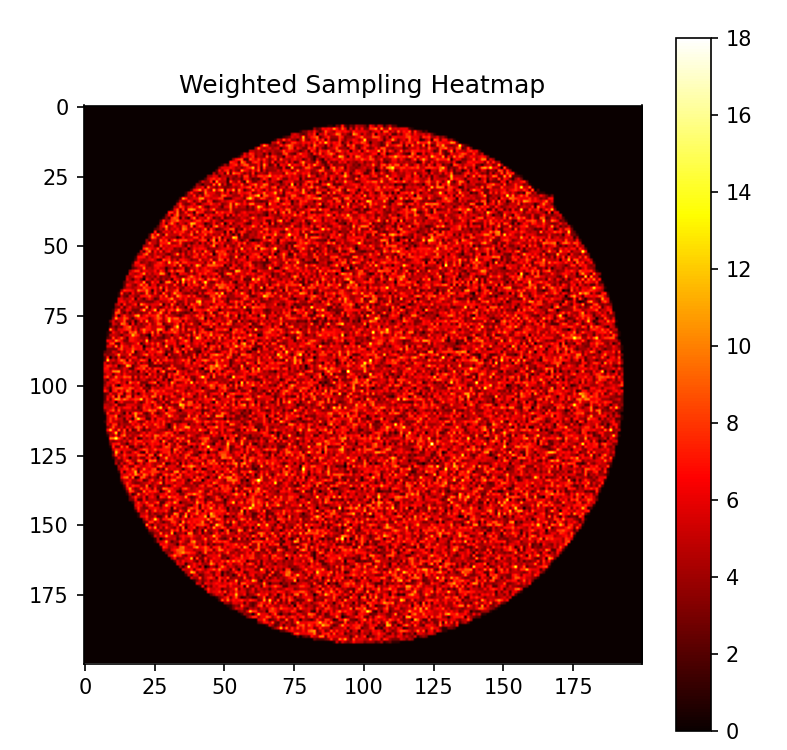
\includegraphics[width=\textwidth]{imaxes/muestraje/random_sampling_heatmap.png}
        \caption{Mapa de calor de muestreo aleatorio}
        \label{fig:random_sampling_heatmap}
    \end{subfigure}
    \hfill
    \begin{subfigure}[b]{0.3\textwidth}
        \centering
        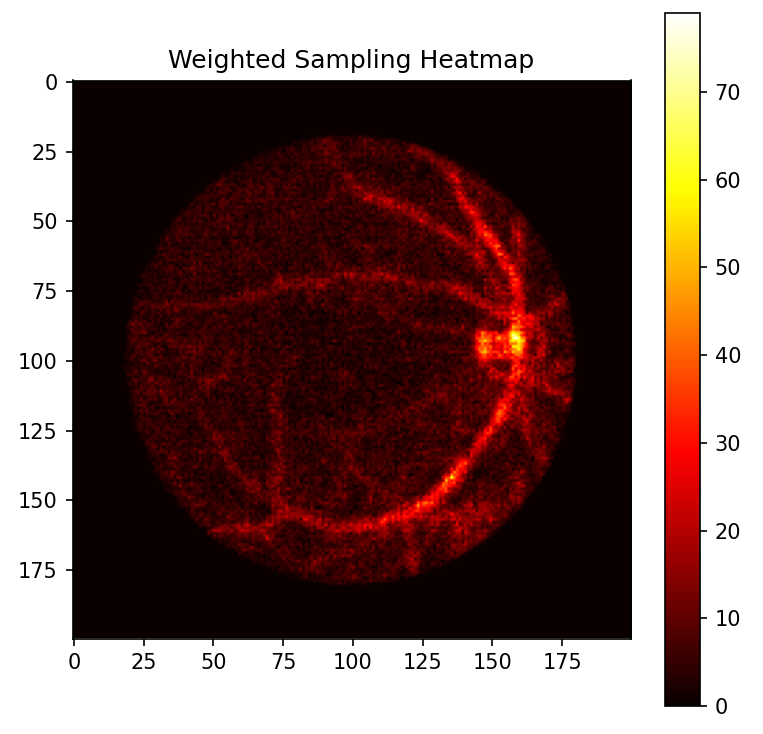
\includegraphics[width=\textwidth]{imaxes/muestraje/weighted_sampling_heatmap.png}
        \caption{Mapa de calor de muestreo ponderado}
        \label{fig:weighted_sampling_heatmap}
    \end{subfigure}
    \hfill
    \begin{subfigure}[b]{0.3\textwidth}
        \centering
        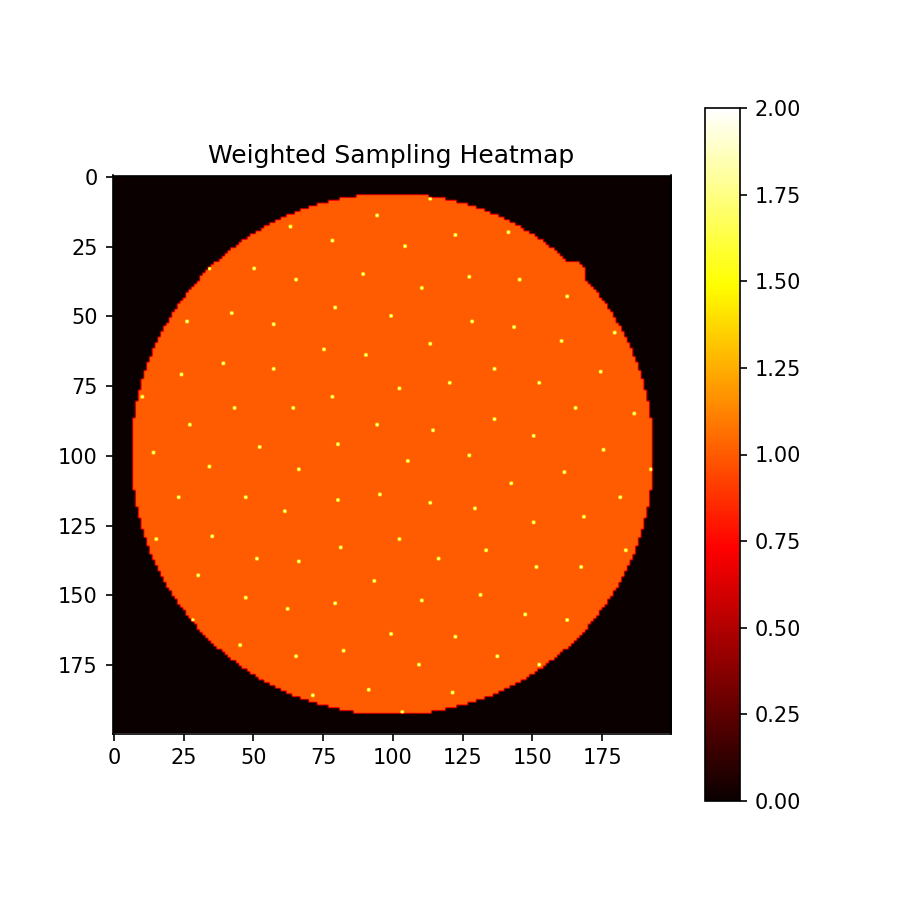
\includegraphics[width=\textwidth]{imaxes/muestraje/uniform_sampling_heatmap.png}
        \caption{Mapa de calor de muestreo uniforme (100 puntos)}
        \label{fig:uniform_sampling_heatmap}
    \end{subfigure}
    \caption{Mapas de calor que ilustran las diferentes estrategias de muestreo implementadas.}
    \label{fig:sampling_heatmaps}
\end{figure}

\subsubsection{Lotería de Inicialización}
\label{subsubsec:loteria_inicializacion}
Otra metodología diseñada fue la implementación de la lotería de inicialización. Esta técnica consiste en probar diferentes inicializaciones aleatorias de los pesos de la red para determinar cuál de ellas resulta más beneficiosa para la convergencia y el rendimiento final del modelo, y seleccionar la mejor inicialización para completar el entrenamiento.

\subsubsection{Ajuste Dinámico del Tamaño del Lote}
\label{subsubsec:axuste_dinamico_batch_size}
Se implementó el ajuste dinámico del tamaño del lote, que consiste en aumentar la cantidad de muestras tomadas por la red a lo largo del entrenamiento. Para llevar a cabo esta estrategia, se dividen las épocas en diferentes fases, donde cada fase hace uso de un tamaño de lote diferente, comenzando normalmente con tamaños más pequeños y aumentándolos progresivamente.

\section{Métodos de Evaluación}
\label{sec:Métodos de Evaluación}

La evaluación del rendimiento del sistema de registro constituye un aspecto fundamental para determinar la eficacia de las modificaciones implementadas.
El proceso de evaluación se divide en dos enfoques complementarios: la evaluación cuantitativa, que emplea métricas numéricas objetivas, y la evaluación cualitativa, que analiza los resultados de forma visual para detectar artefactos o deformaciones no deseadas que puedan escapar a las métricas numéricas.

Ambas evaluaciones son necesarias para obtener una visión completa de la calidad del registro, ya que la evaluación cuantitativa puede no ser suficiente para detectar problemas visuales que no se reflejen en las métricas.

\subsection{Evaluación Cuantitativa}\label{subsec:Avaliación Cuantitativa}

Utilizamos como método de evaluación cuantitativa el propuesto por FIRE \cite{FIRE}
generando un gráfico donde el eje x representa el valor del límite de error y el eje y muestra el porcentaje de pares de imágenes que fueron registrados con éxito para cada límite de error.

El error de registro se calcula mediante la distancia euclidiana media entre los puntos correspondientes en las imágenes fija y móvil:

\begin{figure}[tbp]
    \centering
    \[
    E = \frac{1}{N} \sum_{i=1}^{N} \left\| p_i^{\text{fixo}} - T(p_i^{\text{móbil}}) \right\|
    \]
    \caption{Cálculo del error de registro mediante la distancia euclidiana.}
    \label{fig:erro_registro}
\end{figure}

donde N es el número de puntos de referencia, p son las coordenadas de los puntos y T es la transformación aplicada.

Cuando el error de registro entre un par de imágenes está por debajo del umbral, se considera que el registro fue exitoso y viceversa. Esto da lugar a una curva monótona y continua que refleja la relación entre la tasa de éxito y la precisión objetivo, evitando así la necesidad de establecer un umbral arbitrario.
Estos gráficos se utilizan para ilustrar la precisión del registro tanto para casos individuales (donde se utilizan el porcentaje de parejas de puntos registrados con éxito)
como para el conjunto completo de datos.
Esta métrica facilita la comparación entre distintos métodos competidores y permite seleccionar el más adecuado según la precisión deseada.

Además, en FIRE la evaluación se segmentará en las 3 categorías de imágenes (S, P y A) para analizar el rendimiento del registro en cada una de ellas, ya que cada categoría presenta diferentes desafíos y características.

Mientras que FIRE ya provee los puntos de referencia para la evaluación, RFMID no lo hace.
Por lo tanto, para RFMID, utilizamos el mismo método de evaluación, pero generando los puntos manualmente de forma que cubran el interior de la máscara de la imagen fija (separados por 50 píxeles entre sí).

\begin{figure}[tbp]
    \centering
    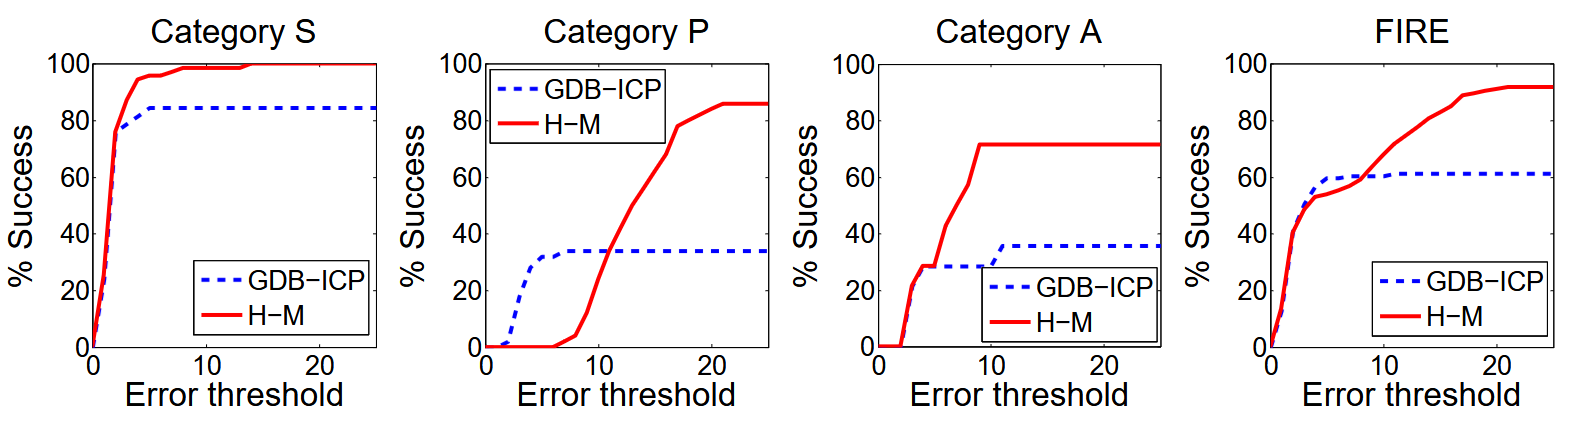
\includegraphics[width=0.8\textwidth]{imaxes/fire_aval.png}
    \caption{Gráfico de evaluación FIRE \cite{FIRE}}
    \label{fig:fire_aval}
\end{figure}

En el caso de RFMiD, dividiremos el conjunto de datos en varias categorías dependiendo de la dificultad del registro, que se calcula mediante la norma de Frobenius de una matriz $A \in \mathbb{R}^{m \times n}$.
Esta es una generalización de la distancia euclidiana aplicada a matrices, donde las imágenes con transformaciones más grandes se consideran más difíciles.

\begin{figure}[tbp]
    \centering
    \[
    \|A\|_F = \sqrt{\sum_{i=1}^{m} \sum_{j=1}^{n} |a_{ij}|^2}
    \]
    \caption{Norma de Frobenius de una matriz $A \in \mathbb{R}^{m \times n}$, donde $a_{ij}$ son los elementos de la matriz $A$.}
    \label{fig:frobenius_norm}
\end{figure}

En algunos casos también utilizaremos la distancia media entre los puntos correspondientes como métrica complementaria para evaluar la calidad del registro, ya que la tasa de éxito puede no ser suficiente para detectar los cambios.

\subsection{Evaluación Cualitativa}
\label{subsec:Avaliación Cualitativa}

En el caso de este trabajo, la evaluación cualitativa cobra gran importancia, ya que en la cuantitativa solo se está comparando sobre un número reducido de puntos en cada pareja de imágenes.
La evaluación visual permite detectar problemas que no se reflejen en las métricas cuantitativas, como artefactos visuales o deformaciones no deseadas,
especialmente en registros que tienen deformaciones locales que pueden no coincidir con ningún punto.

En el caso del dataset FIRE \cite{FIRE}, la evaluación visual es especialmente relevante, ya que tan solo se proporcionan 10 puntos de referencia por imagen, que pueden no ser suficientes para evaluar la calidad del registro en muchas zonas de la imagen.
Ya que en RFMID \cite{RFMiD} se utilizan puntos de referencia generados manualmente que cubren toda la imagen, la evaluación visual es algo menos relevante, ya que es más probable que una deformación local incorrecta sea detectada por algún punto y se vea reflejado en las métricas.

Con el objetivo de identificar fácilmente los distintos artefactos visuales o transformación no realista, se utilizan diferentes herramientas como la composición de imágenes, la visualización de los vectores de desplazamiento y la comparación de imágenes antes y después del registro.
En la figura \ref{fig:visex} se pueden observar algunos ejemplos de estas.

\begin{figure}[tbp]
    \centering
    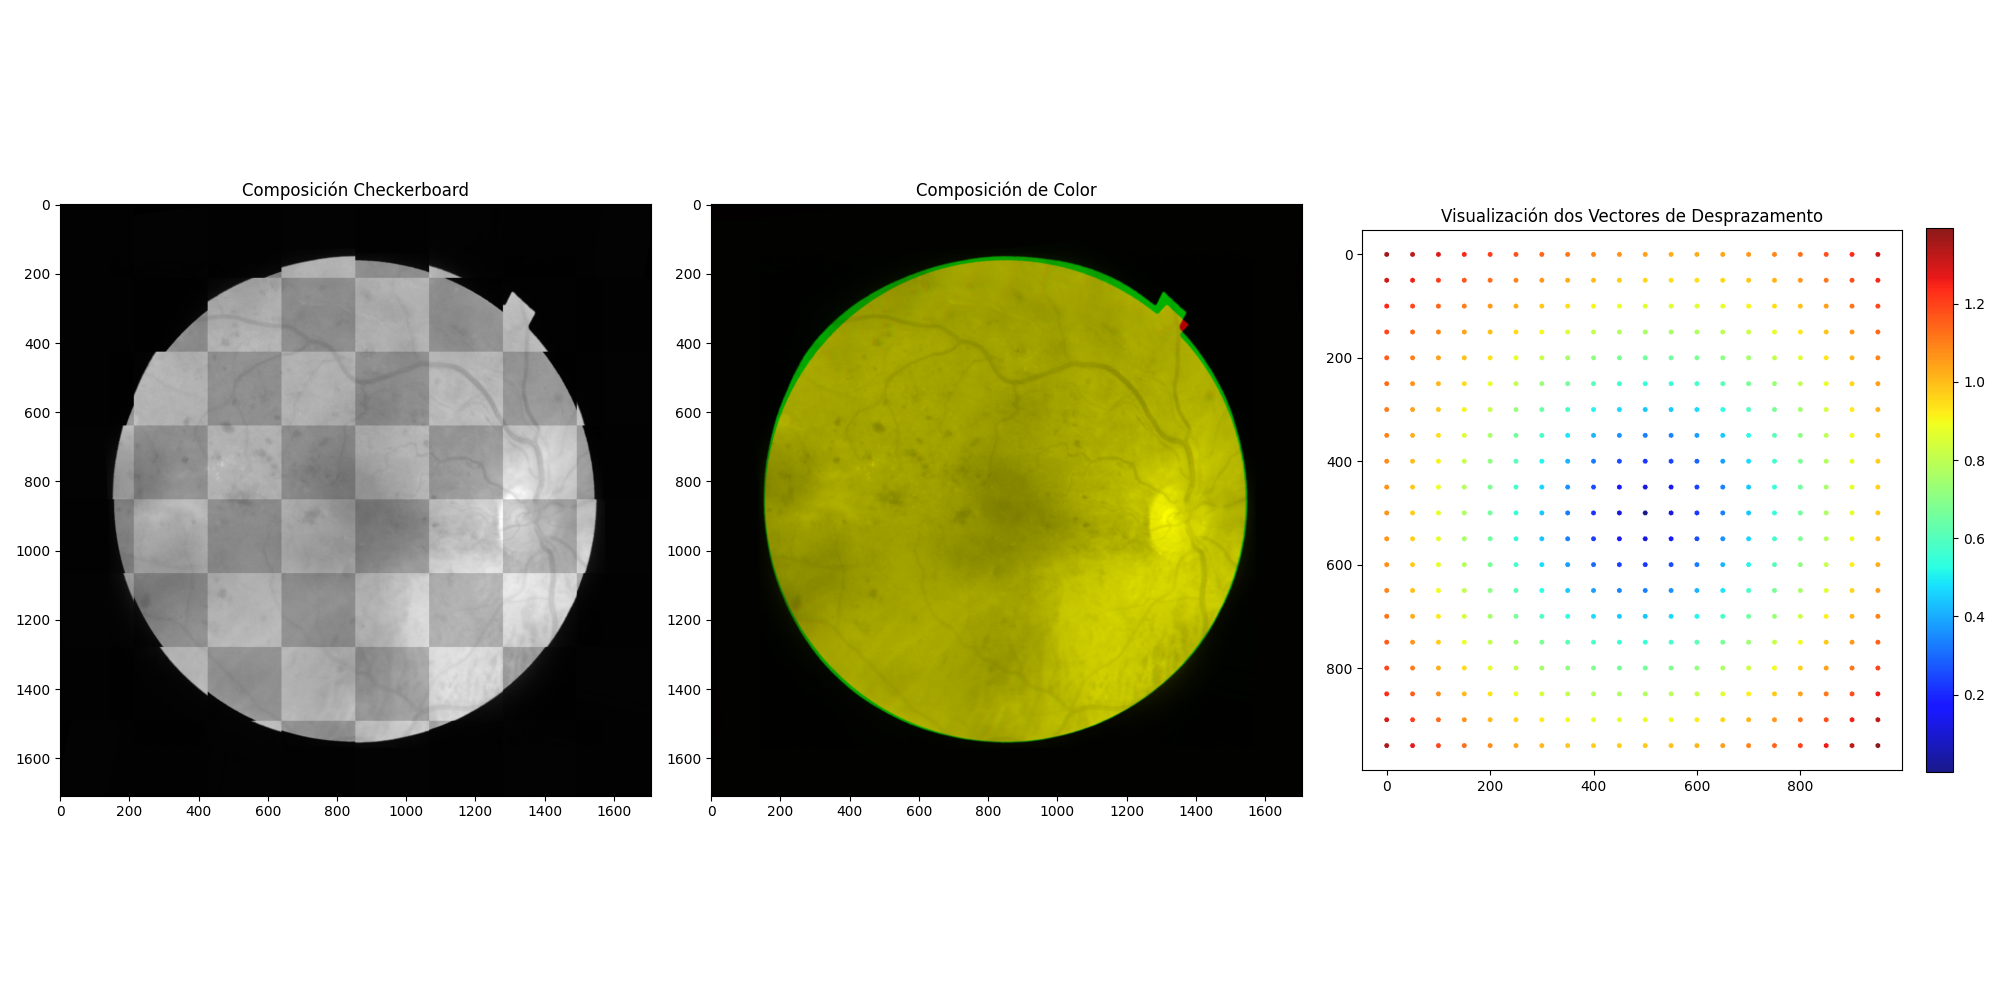
\includegraphics[width=0.9\textwidth]{imaxes/visex.png}
    \caption{Ejemplos de evaluación visual: (a) Composición de imágenes en checkerboard, (b) Composición de imágenes por color, (c) Visualización de los vectores de desplazamiento.}
    \label{fig:visex}
\end{figure}